\documentclass{article}

\usepackage{graphicx}
\usepackage{caption}

\title{Configuración de entorno de desarrollo}
\author{EDER OMAR ZUÑIGA ZAVALA}
\date{Septiembre 2026}

\begin{document}

\maketitle

\newpage

\section{Configuración del entorno}

\subsection{Instalación del módulo Venv de Python}

\begin{flushleft}
    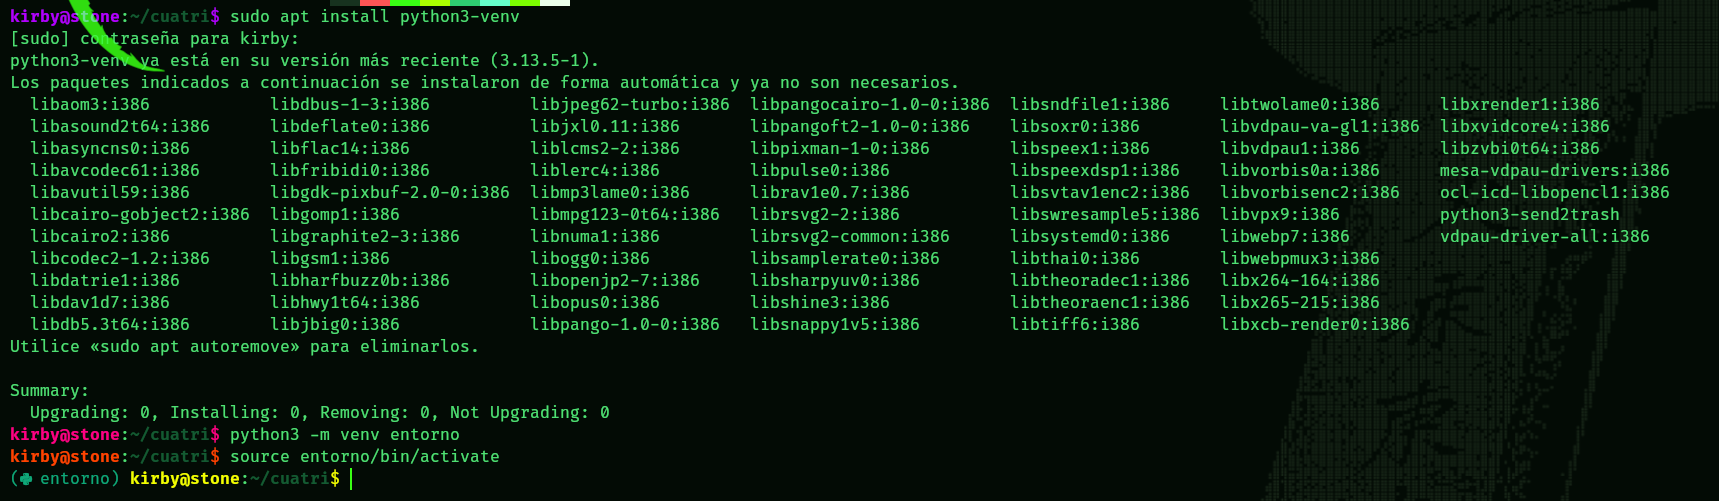
\includegraphics[width=1.8\textwidth]{img/1.png}
\end{flushleft}

\subsection{Ejecución del script en Python}

\begin{flushleft}
    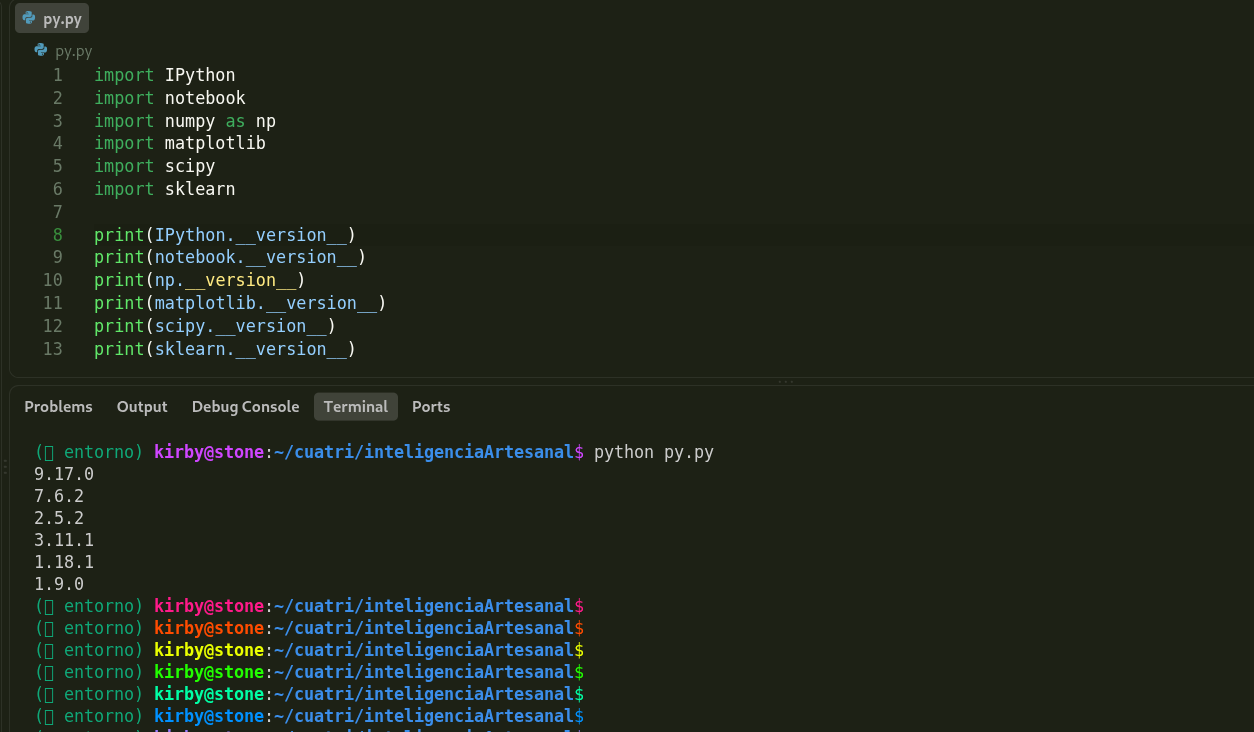
\includegraphics[width=1.3\textwidth]{img/2.png}
\end{flushleft}


\subsection{breve resumen}

\begin{flushleft}
    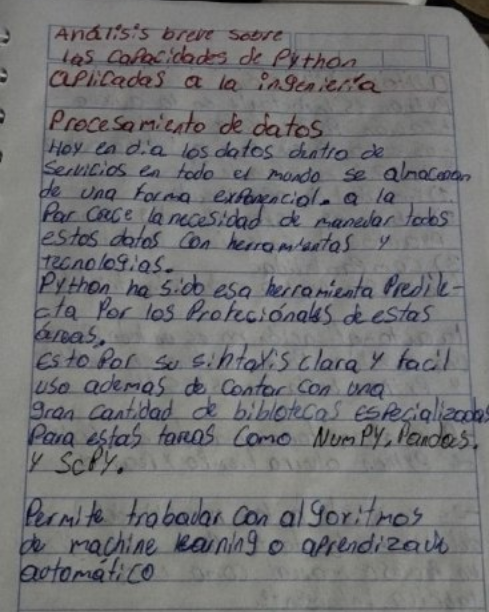
\includegraphics[width=1.3\textwidth]{img/3.png}
    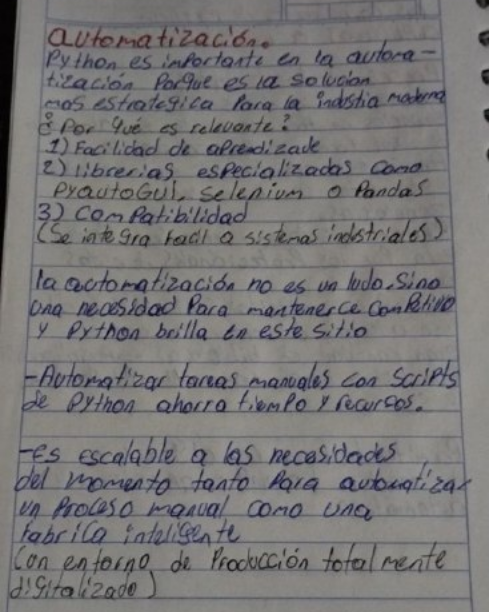
\includegraphics[width=1.3\textwidth]{img/4.png}
    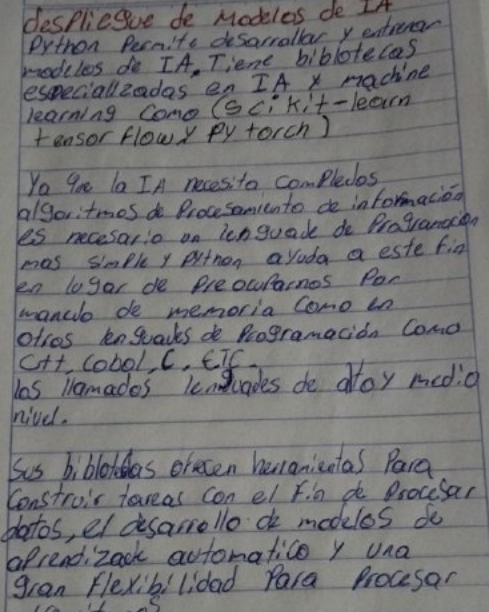
\includegraphics[width=1.3\textwidth]{img/5.png}
\end{flushleft}

\end{document}